Gruppen vil udvikle et system til vanding af golfbaner. I forbindelse med stigende temperaturer bliver det mere kritisk, at vandingen af golfbaner sker på de rigtige tidspunkter, for at holde banen spilbar. For at spare på ressourcerne er det også kritisk, ikke at spilde store mængder vand, på vanding af områder som ikke trænger til det. 

Med et system af intelligente enheder der arbejder autonomt, men som modtager indstillinger for vandingen fra en master, styres vandingen på hele golfbanen centralt. På denne måde sparer man arbejdstid for greenkeeperen og vandingen sker kun når det er nødvendigt. Systemet kaldes for EasyWater8000. 
Normalt vil man placere en af disse enheder ved hvert hul på golfbanen og lave et netværk af sensorer lokalt til denne enhed. Enheden kan herved overvåge området og vande hvis nødvendigt. Alle enhederne forbindes til et netværk, som er koblet sammen med en masterenhed. Grænseværdierne, for f.eks. jordfugtigheden, der afgør hvornår enheden, skal påbegynde vanding kommer fra master og styres igennem denne af greenkeeperen. 


\begin{figure}[ht] \centering
\fbox{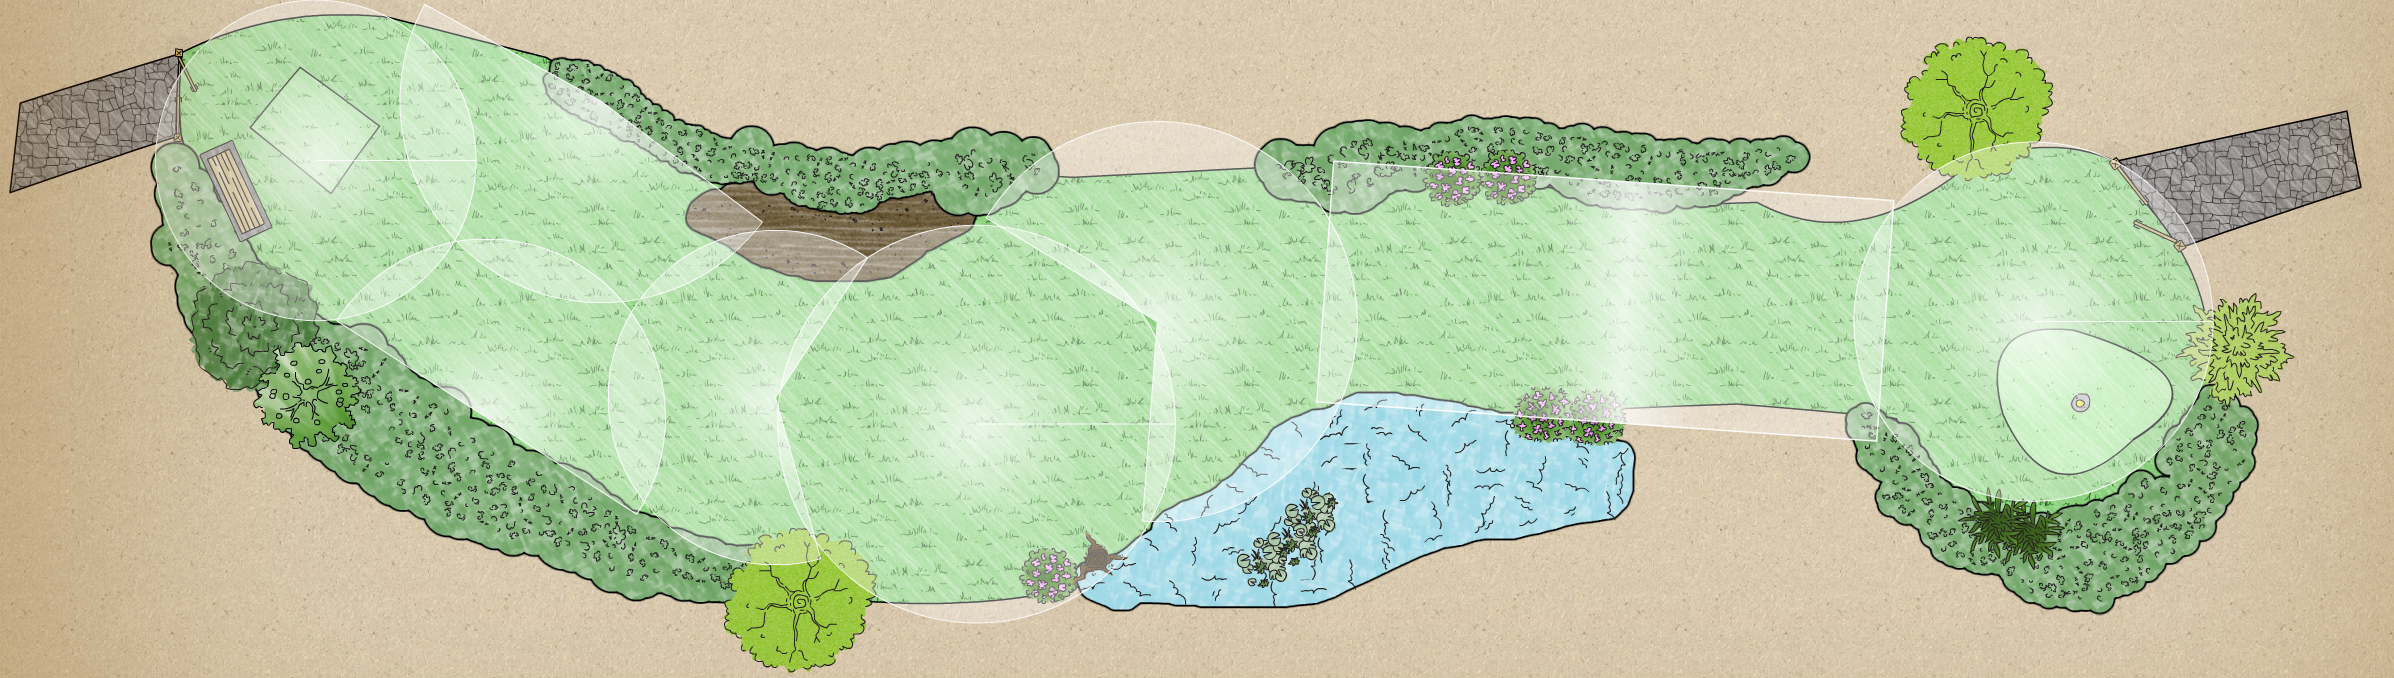
\includegraphics[height=4.1cm]{filer/indledning/billeder/hul_med_sprinkler}}
\caption{Overblik af golfhul med distribuerede sprinklere}
\label{fig:systemoverblik}
\end{figure}

Figur \ref{fig:systemoverblik} illustrerer et hul på en given golfbane. Dette hul er inddelt i 11 områder, med hver sin sprinkler. Spinklere er markeret ved halv til helcirkler på figuren. Til venstre på figuren ses tee-stedet med tilhørende indgang. Ved denne indgang er der placeret en bevægelsessensor, som sørger for at der ikke kan vandes på banen, når der er spillere. 

Oversigt over blokkene i systemet kan ses i figur \ref{fig:bloksystemoverblik}. De tre hovedbegreber for systemet er master, som er hovedenheden baseret på Devkit8000. Enhed som er de autonome undersystemer på hvert hul, hvor hovedenheden er PSoC4, og Komponentpakker som er et begreb for pakken med temperatur- og fugtsensor samt sprinkler. Disse er distribueret ud på selve golfhullet.

\begin{figure}[ht] \centering
\fbox{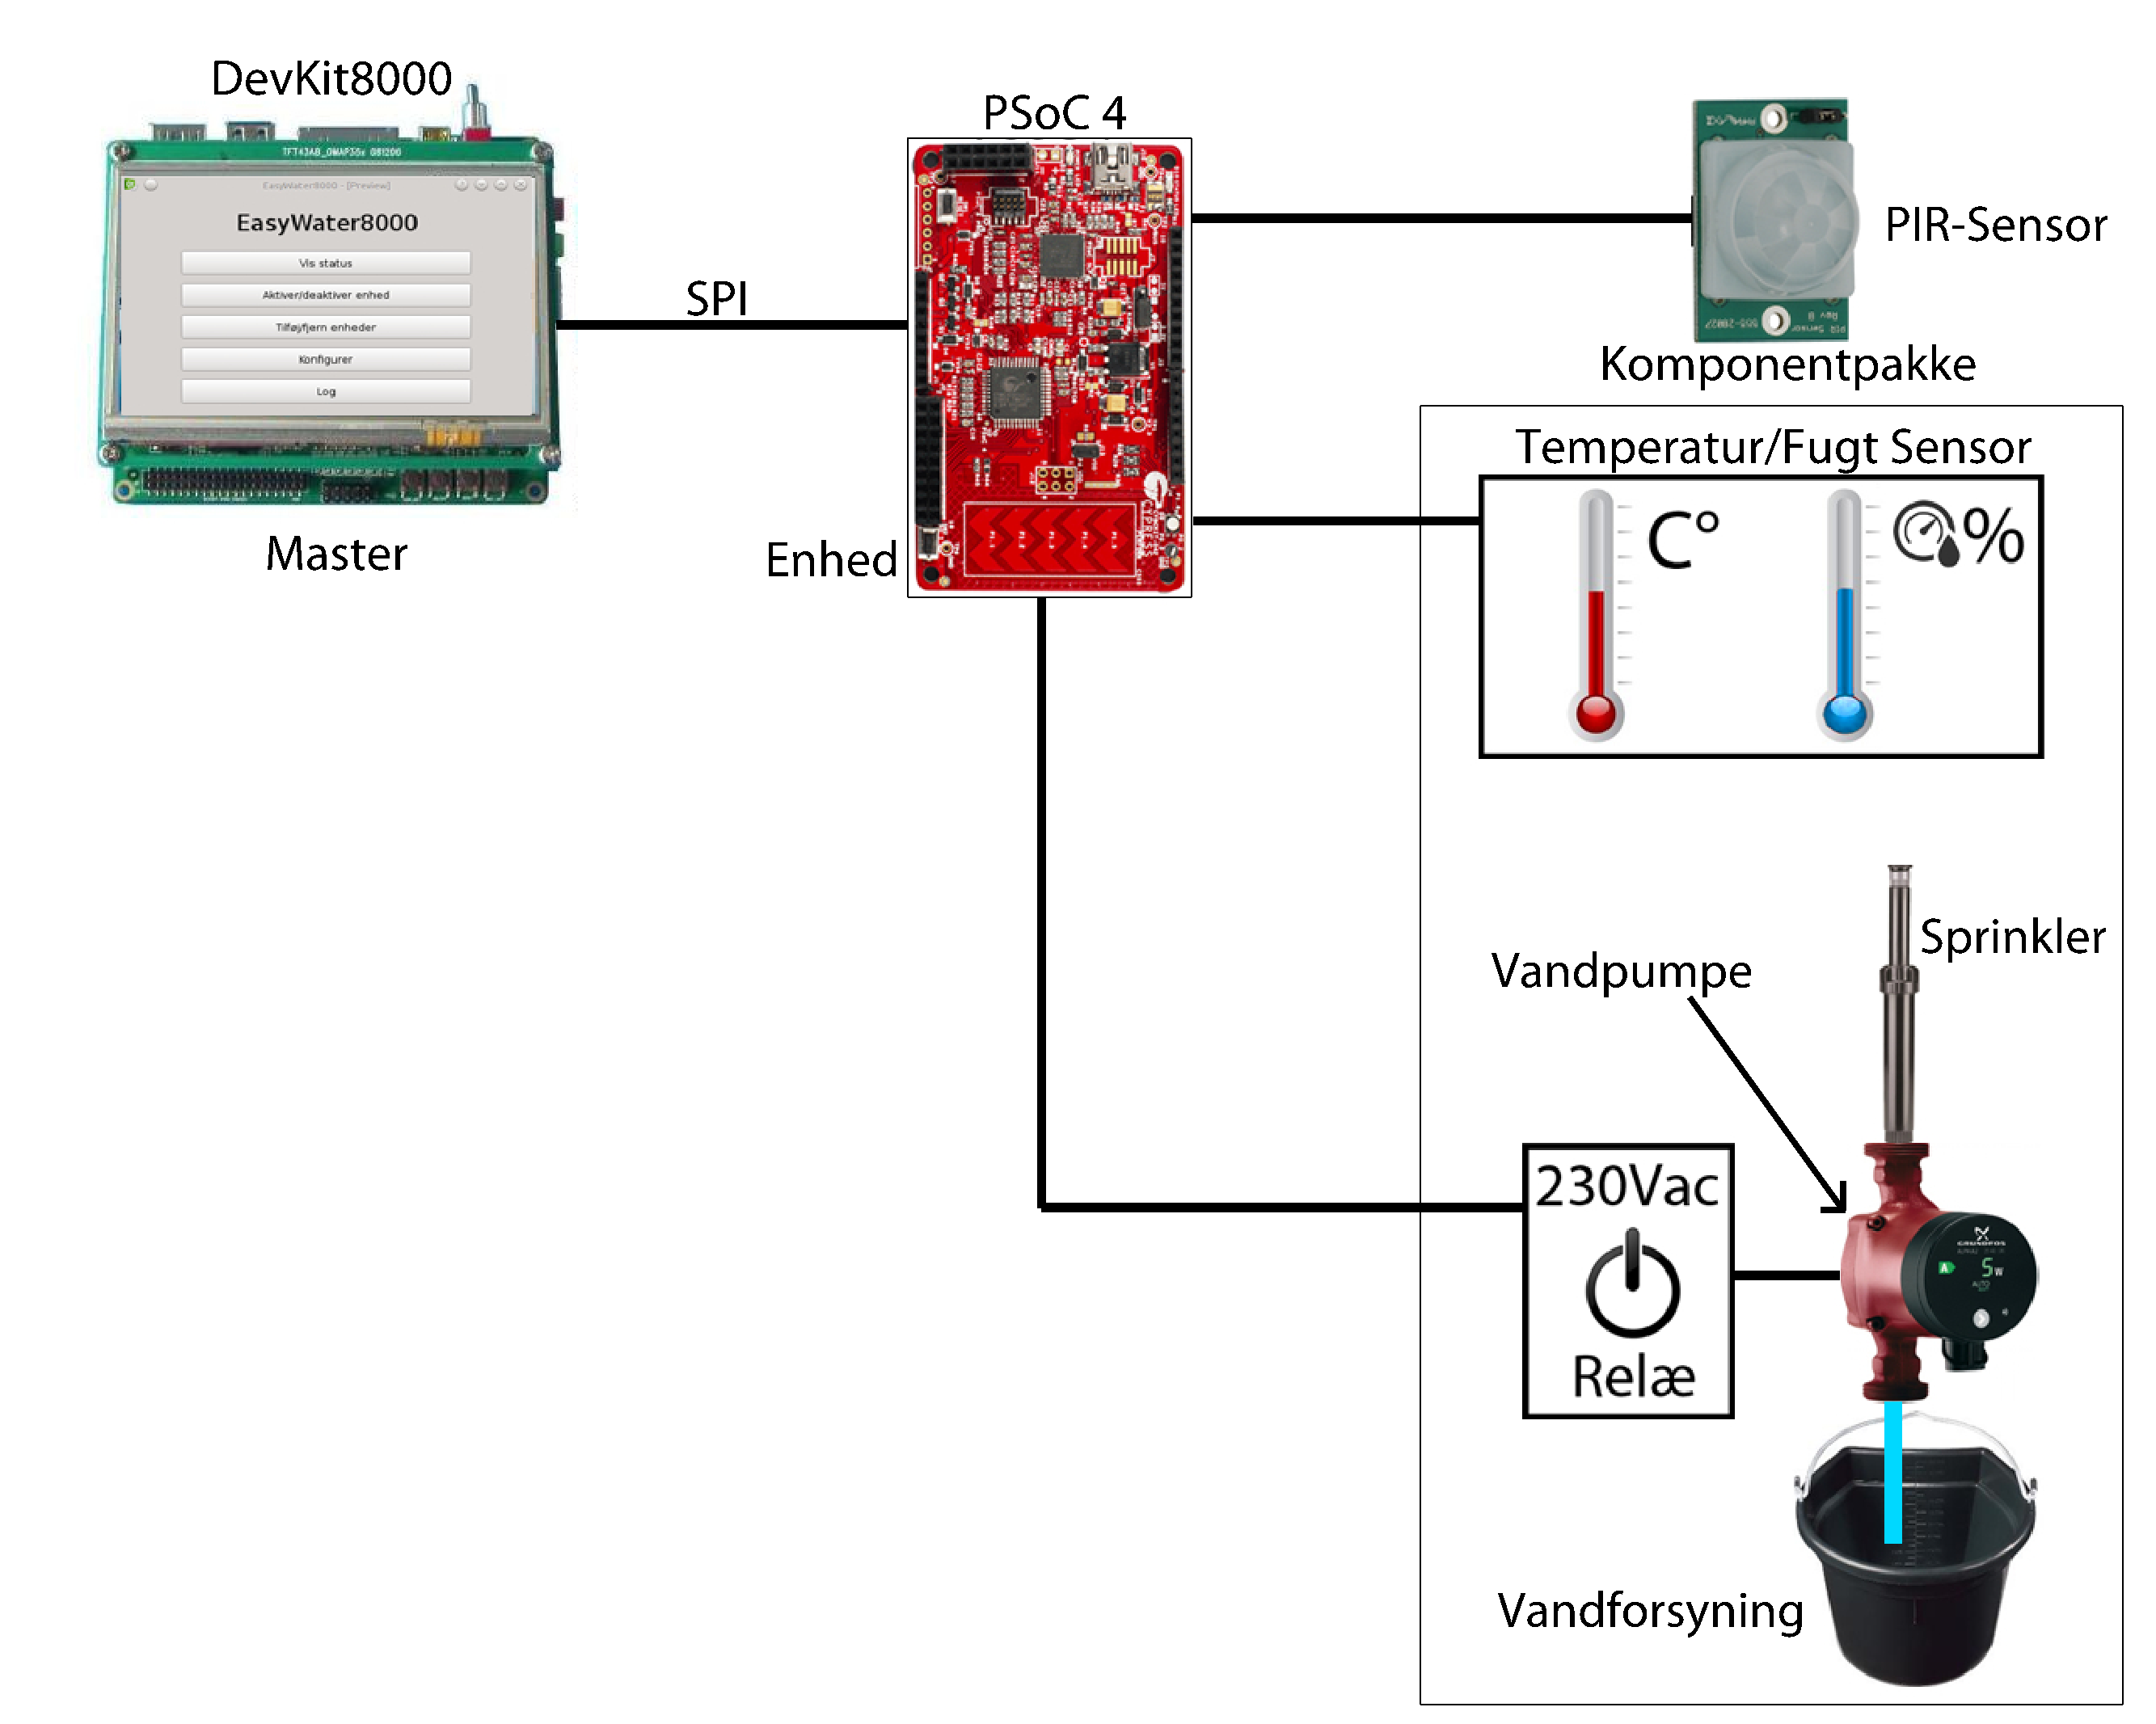
\includegraphics[height=10cm]{filer/indledning/billeder/vandingssystem}}
\caption{Konceptuelt systemoverblik med de benyttede blokke}
\label{fig:bloksystemoverblik}
\end{figure}

En Enhed består altså af:
\begin{enumerate}
\item Fugtighedssensor(er)
\item Temperatursensor(er)
\item Bevægelsessensor(er) 
\item Sprinkler(e)
\item PSoC controller board
\end{enumerate}

Fugt- og temperatursensorerne registrerer banens behov for vanding. Bevægelsessensoren registrerer om der er spillere på det pågældende hul. Sprinkleren sørger for vandingen når der skal vandes. Denne skjules nede i græsset og kommer op når vandingen skal være aktiv.
PSoC4 controller-boardet bliver hjernen i Enheden. Denne holder styr på de generelle funktioner for Enheden så som udlæsning af data, aktivering af sprinkler m.v.